\documentclass[11pt,a4paper]{article}
\usepackage[UTF8]{ctex}
\usepackage{geometry}
\usepackage{graphicx}
\usepackage{xcolor}
\usepackage{hyperref}
\usepackage{fancyhdr}
\usepackage{titlesec}
\usepackage{booktabs}
\usepackage{longtable}
\usepackage{caption}

\geometry{left=2.5cm,right=2.5cm,top=2.5cm,bottom=2.5cm}
\hypersetup{colorlinks=true,linkcolor=blue,urlcolor=blue}

\titleformat{\section}{\large\bfseries\color{blue!80!black}}{}{0em}{}[\vspace{0.3em}\hrule]
\titleformat{\subsection}{\normalsize\bfseries}{}{0em}{}

\pagestyle{fancy}
\fancyhf{}
\fancyhead[L]{\small 课程素材库系统 · 设计手册}
\fancyhead[R]{\small v1.0}
\fancyfoot[C]{\thepage}

\begin{document}

\title{\vspace{-2cm}\textbf{课程素材库系统设计手册}}
\author{基于程老师课程素材需求}
\date{\today}
\maketitle

\section{概述}

本手册描述课程素材库系统的设计方案，覆盖程老师对书法课程素材管理的核心需求。
系统采用「素材分类→素材→标签」三级结构，支持视频、音频、图片、文档等多类型素材的统一管理。

\subsection{设计目标}

\begin{itemize}
  \item 素材按分类归档（书写肌能/规范楷书/文化素养）
  \item 多维度标签筛选（班型/技法/难度）
  \item 按素材类型筛选（视频/音频/图片/文档）
  \item 教师自由组合素材生成课程
  \item 素材可跨课程复用
\end{itemize}

\section{数据结构}

\subsection{ER 关系}

\begin{verbatim}
素材分类 1──N 素材 N──N 标签
                │
                N
              课程 (引用素材的有序集合)
\end{verbatim}

\subsection{核心表结构}

\textbf{素材分类表 (course\_material\_category)}:

\begin{tabular}{lll}
\toprule
字段 & 类型 & 说明 \\
\midrule
id & VARCHAR & 主键 \\
name & VARCHAR & 分类名称（如"书写肌能素材库"） \\
sort\_order & INT & 排序 \\
\bottomrule
\end{tabular}

\vspace{0.5em}
\textbf{素材表 (course\_material)}:

\begin{tabular}{lll}
\toprule
字段 & 类型 & 说明 \\
\midrule
id & VARCHAR & 主键 \\
category\_id & VARCHAR & 所属分类 \\
title & VARCHAR & 素材标题 \\
material\_type & VARCHAR & 类型：video/audio/doc/image \\
file\_url & VARCHAR & 存储路径 \\
file\_size & BIGINT & 文件大小（字节） \\
duration\_seconds & INT & 视频/音频时长 \\
tags & JSONB & 标签阵列 \\
created\_at & TIMESTAMP & 创建时间 \\
\bottomrule
\end{tabular}

\vspace{0.5em}
\textbf{课程-素材关联表 (course\_material\_rel)}:

\begin{tabular}{lll}
\toprule
字段 & 类型 & 说明 \\
\midrule
course\_id & VARCHAR & 课程ID \\
material\_id & VARCHAR & 素材ID \\
sort\_order & INT & 排序序号 \\
\bottomrule
\end{tabular}

\section{搜索与筛选}

\subsection{搜索维度}

系统支持以下搜索与筛选维度：

\begin{itemize}
  \item \textbf{关键词搜索}：按素材标题搜索
  \item \textbf{素材类型筛选}：视频 / 音频 / 图片 / 文档
  \item \textbf{标签筛选}：班型标签（启蒙/基础/精修/素养）、技法标签（笔画/结构/章法）、难度标签（入门/进阶/高阶）
  \item \textbf{分类浏览}：按素材分类目录浏览
\end{itemize}

\subsection{搜索逻辑}

\begin{verbatim}
SELECT * FROM course_material
WHERE category_id = ?
  AND material_type IN (?)
  AND tags @> ARRAY[?]::VARCHAR[]
  AND title ILIKE '%keyword%'
ORDER BY created_at DESC
\end{verbatim}

\section{原型界面}

\subsection{素材库主页}

素材库主页包含：顶部搜索栏、素材类型筛选标签（全部/视频/文档/音频）、分类切换 tabs、素材卡片列表。

\begin{figure}[h]
\centering
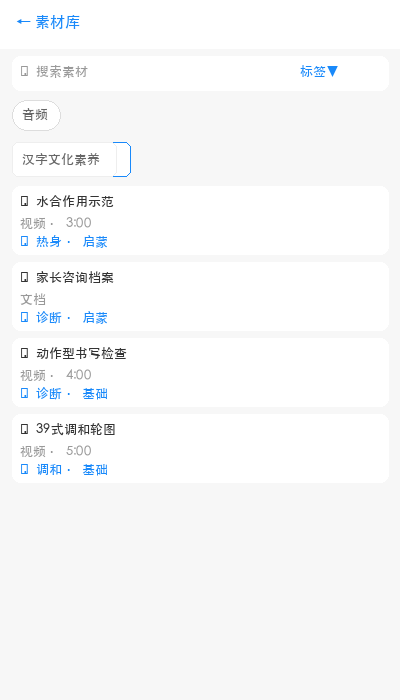
\includegraphics[width=0.55\textwidth]{screenshots/proto_material_library.png}
\caption{素材库主页原型}
\label{fig:library}
\end{figure}

\subsection{课程编辑页}

教师在编辑课程时，可以从底部弹出的素材选择器中选择已有素材，按序添加到课程内容区。

\begin{figure}[h]
\centering
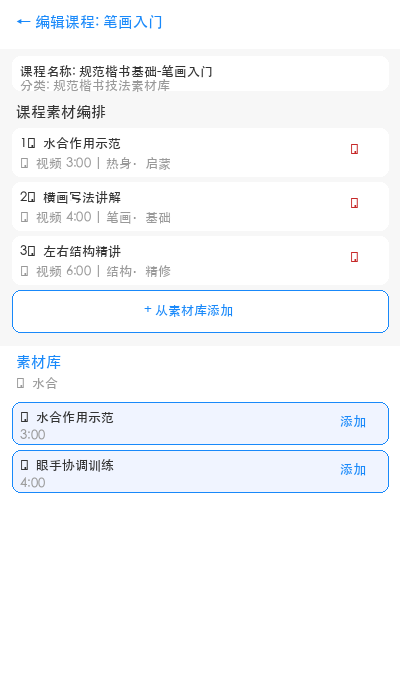
\includegraphics[width=0.55\textwidth]{screenshots/proto_course_edit.png}
\caption{课程编辑页（素材选择器）原型}
\label{fig:edit}
\end{figure}

\section{组课流程}

教师通过以下步骤完成课程创建：

\begin{enumerate}
  \item 选择素材分类（如"规范楷书技法素材库"）
  \item 按标签筛选素材（如勾选"笔画"+"基础"）
  \item 按类型筛选（如只显示"视频"）
  \item 选择素材添加到课程列表中
  \item 拖拽调整素材顺序
  \item 保存生成课程
\end{enumerate}

\subsection{实际数据示例}

\begin{verbatim}
课程: "规范楷书基础 - 笔画入门"
分类: 规范楷书技法素材库

素材列表:
  1. 水合作用示范 (视频 3:00) [热身·启蒙]
  2. 横画写法讲解 (视频 4:00) [笔画·基础·入门]
  3. 竖画写法讲解 (视频 3:00) [笔画·基础·入门]
  4. 笔画专项练习 (文档) [笔画·基础]
\end{verbatim}

\section{实施建议}

\begin{enumerate}
  \item 素材类型枚举：video / audio / doc / image，前端根据类型显示不同图标和元数据
  \item 标签字段使用 PostgreSQL JSONB 或 ARRAY，支持 GIN 索引加速筛选
  \item 视频/音频文件上传时提取时长元数据
  \item 素材选择器组件设计为弹窗模式，不跳转页面
  \item 现有 JSONB 嵌入的素材数据提供迁移工具
\end{enumerate}

\vfill
\begin{center}
\small \textcolor{gray}{—— 课程素材库系统设计手册 ——}
\end{center}

\end{document}
